\documentclass[12pt,a4paper]{article}
\usepackage[polish]{babel}
\usepackage[T1]{fontenc}
\usepackage{lmodern}
\usepackage[utf8x]{inputenc}
\usepackage{hyperref}
\usepackage{url}
\usepackage{graphicx}
\usepackage{listings}
%\usepackage{xcolor}
\usepackage{color}
\usepackage{float}
\usepackage{multicol}
\usepackage{tikz}

\usetikzlibrary{shapes.geometric, arrows}
\tikzstyle{startstop} = [rectangle, rounded corners, minimum width=3cm, minimum height=1cm,text centered, draw=black, fill=red!30]
\tikzstyle{io} = [trapezium, trapezium left angle=70, trapezium right angle=110, minimum width=3cm,text width=4cm, minimum height=1cm, text centered, draw=black, fill=blue!30]
\tikzstyle{process} = [rectangle, minimum width=3cm, minimum height=1cm, text centered, text width=4cm, draw=black, fill=orange!30]

\tikzstyle{decision} = [diamond, minimum width=3cm, minimum height=1cm, text centered, draw=black, fill=green!30]
\tikzstyle{arrow} = [thick,->,>=stealth]

\addtolength{\hoffset}{-1.5cm}
\addtolength{\marginparwidth}{-1.5cm}
\addtolength{\textwidth}{3cm}
\addtolength{\voffset}{-1cm}
\addtolength{\textheight}{2.5cm}
\setlength{\topmargin}{0cm}
\setlength{\headheight}{0cm}

%\lstset{
%    numbers=left,
%    breaklines=true,
%    tabsize=2,
%    basicstyle=\ttfamily,
%    frame=lr,
%    rulecolor=\color{blue!80!black},
%    language=[Sharp]C
%}
\definecolor{bluekeywords}{rgb}{0,0,1}
\definecolor{greencomments}{rgb}{0,0.5,0}
\definecolor{redstrings}{rgb}{0.64,0.08,0.08}
\definecolor{xmlcomments}{rgb}{0.5,0.5,0.5}
\definecolor{types}{rgb}{0.17,0.57,0.68}
\lstset{language=[Sharp]C,
captionpos=b,
frame=lines,
showspaces=false,
showtabs=false,
breaklines=true,
showstringspaces=false,
breakatwhitespace=true,
escapeinside={(*@}{@*)},
commentstyle=\color{greencomments},
morekeywords={partial, var, value, get, set},
keywordstyle=\color{bluekeywords},
stringstyle=\color{redstrings},
basicstyle=\ttfamily\small,
tabsize=4,
}

\begin{document}
	
	\title{Heurystyczne Metody Optymalizacji\\ Informatyka, sem V \\{Dokumentacja projektu Unity Neural Network Car}}
	\author{Artur Bednarczyk, Dawid Grajewski, grupa A}
	\date{\today}
	
	\maketitle
	\newpage
	\tableofcontents
	\newpage
	\section{Część I}
	\subsection{Opis programu}
	Unity Neural Network Car to symulacja samochodu poruszającego się po torze. Jednak nie tylko użytkownik może kontrolować pojazd, a również sztuczna inteligencja. Implementacja zaawansowanej technologii pozwoliła na ,,nauczenie'' samochodu w jaki sposób przejechać przez cały tor i nie rozbić się na najbliższym zakręcie.
	\begin{figure}[H]
	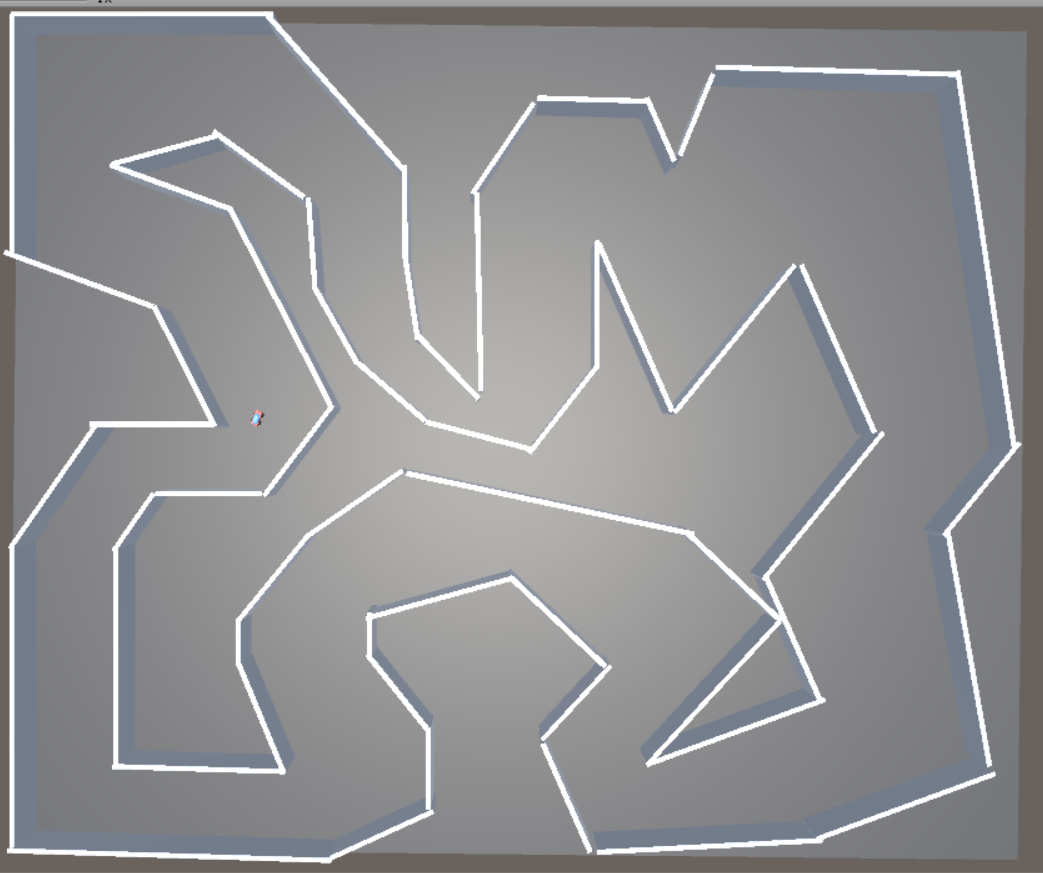
\includegraphics[width=\textwidth]{car}
	\centering
	\end{figure}
	\subsection{Instrukcja obsługi}
	Uruchamiamy aplikację i możemy obserwować ruch pojazdu.
	\subsection{Dodatkowe informacje}
	Projekt został wykonany z wykorzystaniem silnika Unity oraz języka C\#.
	\newpage
	\section{Część II}
	\subsection{Opis działania} 
\subsubsection{Sieć neuronowa}
Sieć neuronowa jest strukturą inspirowaną budową naturalnych neuronów, łączących je synaps oraz układów nerwowych. Wykorzystana w projekcie sieć jest wielowarstwową siecią jednokierunkową korzystającą z algorytmu propagacji wstecznej.
\subsubsection{Budowa sieci}
Wykorzystana sieć składa się z trzech głównych warstw.
\begin{itemize}
	\item Warstwa wejścia.
	\item Warstwy ukryte.
	\item Warstwa wyjścia.
\end{itemize}
\paragraph*{Warstwa wejścia} Każdy neuron tej warstwy przekazuje do warstwy ukrytej początkowe wartości.
\paragraph*{Warstwy ukryte} Tutaj dzieje się wszystko co najważniejsze. Synapsy między neuronami mają przypisane wagi, które początkowo są losowe. W ramach uczenia się, wagi są dostosowywane tak, aby rezultat końcowy był jak najbliżej spodziewanego.
\paragraph*{Warstwa wyjścia} To tutaj nauczona już sieć daje nam wynik.
\subsubsection{Uczenie sieci}
Uczenie sieci jest realizowane poprzez podanie jej zestawu danych wejściowych oraz spodziewanych wyników. W tym projekcie wykorzystano metody takie jak:
\begin{itemize}
\item Propagacja Wsteczna
\item Biases
\item Momentum
\item Współczynnik uczenia
\end{itemize}

\paragraph*{Propagacja wsteczna} to podstawowy algorytm uczenia nadzorowanego wielowarstwowych, jednokierunkowych sieci neuronowych. Dzięki wstecznej propagacji błędu możemy dobrać odpowiednie wagi we wszystkich warstwach sieci. Początkowo dla losowych wag obliczane są błędy, czyli różnica między odpowiedzią obliczoną a spodziewaną, które następnie są propagowane do wcześniejszych warstw. Wagi zostają modyfikowane na podstawie błędu i obliczonych danych. Algorytm jest zostaje zatrzymany, gdy średnia wartość błędu przestanie maleć.
\paragraph*{Biases} Są to wartości, które pozwalają na przesunięcie funkcji aktywacji w sposób, na który zmiana wagi nie pozwala. Przykład funkcji bez bias:
\begin{figure}[H]
\centering
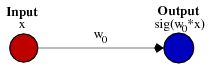
\includegraphics[scale=0.7]{biases_01}
\caption{https://stackoverflow.com/questions/2480650/role-of-bias-in-neural-networks}
\end{figure}
\begin{figure}[H]
\centering
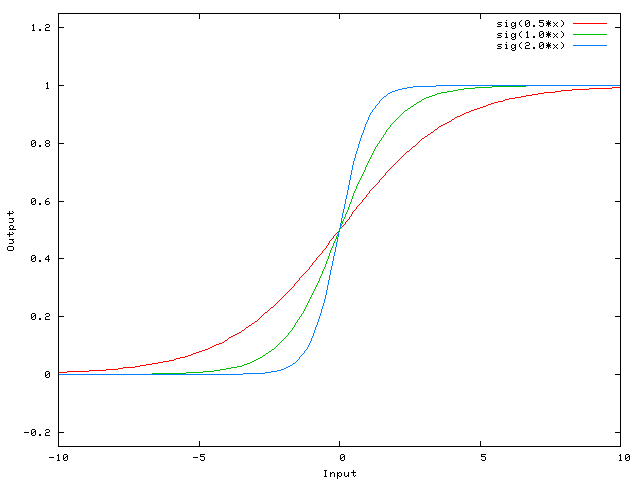
\includegraphics[scale=0.5]{biases_02}
\caption{https://stackoverflow.com/questions/2480650/role-of-bias-in-neural-networks}
\end{figure}\clearpage
Przykład funkcji z bias:
\begin{figure}[H]
\centering
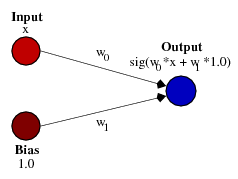
\includegraphics[scale=0.7]{biases_03}
\caption{https://stackoverflow.com/questions/2480650/role-of-bias-in-neural-networks}
\end{figure}
\begin{figure}[H]
\centering
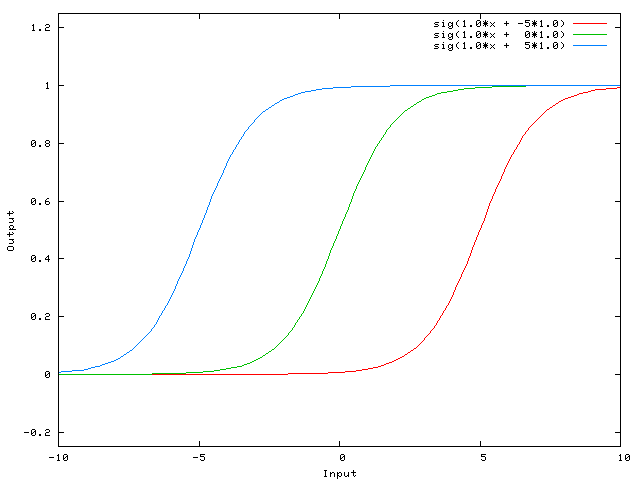
\includegraphics[scale=0.5]{biases_04}
\caption{https://stackoverflow.com/questions/2480650/role-of-bias-in-neural-networks}
\end{figure}
Wykorzystanie tego jest konieczne aby uczenie zostało zrealizowane z prawidłowymi wynikami.
\paragraph*{Momentum} Jest to współczynnik odpowiadający za dodanie ułamka poprzedniej wagi do aktualnej. Używany jest aby zapobiec zbieżności do lokalnego minimum lub punktu siodłowego. Wysoka wartość tego współczynnika przyspiesza proces konwergencji, jednakże zbyt wysoka może spowodować, że cały system stanie się niestabilny, a zbyt niska spowolni proces uczenia.
\paragraph*{Współczynnik uczenia} to współczynnik odpowiadający za to jak duże są zmiany wag oraz biasów.
\subsubsection{Funkcja Aktywacji}
Wartość wyjścia neuronów jest obliczana za pomocą funkcji aktywacji. W tym projekcie została użyta funkcja sigmoidalna:
$$ S(x) = \frac{1}{1+e^{-x}} = \frac{e^x}{e^x+1} $$
\begin{figure}[H]
\centering
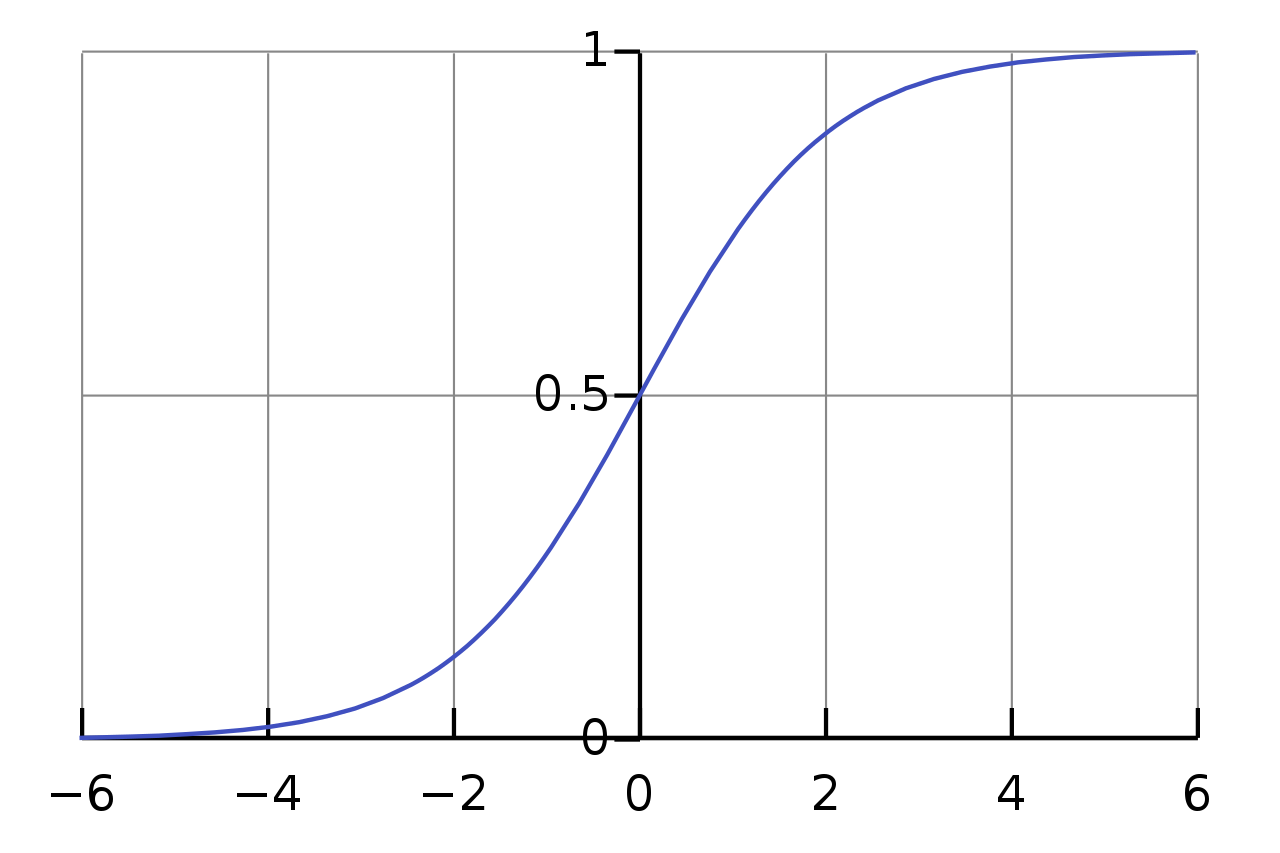
\includegraphics[scale=0.3]{sigmoid}
\caption{https://en.wikipedia.org/wiki/Sigmoid\_function}
\end{figure}
Funkcja ta przyjmuje wartości od 0 do 1.
	\subsection{Algorytm}
	\begin{figure}[H]
		\centering

	\begin{tikzpicture}[node distance=2cm]
		\node (start) [startstop] {START};
		\node (dec1) [decision, below of=start, yshift=-1.0cm]{Jeśli sieć nauczona.};
		\node (in1) [io, left of=dec1, xshift=-4.3cm]{Pobranie danych treningowych};
		\node (pro1) [process, below of=in1]{Uczenie sieci};
		\node (out1) [io, below of=pro1]{Zapis danych};
		\node (pro2) [process, below of=out1] {Podłączenie sieci do auta};
		\node (pro3) [process, below of=pro2] {Auto jedzie.} ;
		\node (stop) [startstop, below of=pro3] {STOP};
		
		
		\draw [arrow](start) -- node {}(dec1);
		\draw [arrow] (dec1) -- node[anchor=south] {Nie} (in1);
		\draw [arrow] (dec1) |- node[anchor=west] {Tak} (pro2);
		\draw [arrow] (in1) -- node {} (pro1);
		\draw [arrow] (pro1) -- node {} (out1);
		\draw [arrow] (out1) -- node {} (pro2);
		\draw [arrow] (pro2) -- node {} (pro3);
		\draw [arrow] (pro3) -- node {} (stop);
	\end{tikzpicture}	\end{figure}\clearpage
	
	\subsection{Bazy danych}
	Zestaw danych wykorzystany do uczenia sieci:
	\begin{multicols}{3}
	\begin{verbatim}
	14.85;14.85;0
15.2;14.53;-0.58
13.32;17.02;1
14.13;15.67;0.91
15.17;14.55;-0.55
11.15;17.01;1
11.61;13.86;0.98
12;12.78;0.65
12.11;12.54;0.41
12.27;12.21;-0.06
9.19;10.16;0.75
11.7;11.57;-0.13
21.19;30.54;1
11.52;13.08;0.92
15.13;14.7;-0.41
13.91;5.75;-1
27.65;7.57;-1
25.97;28.01;0.97
2.45;34.22;1
6.81;25.24;1
16.07;9.18;-1
8.77;28.54;1
53.54;16.19;-1
14.85;14.85;0
11.91;20.92;1
15.48;13.44;-0.97
11.55;42.66;1
9.13;57.46;1
11.39;8.89;-0.99
8.77;17.61;1
6.76;11.94;1
9.29;17.88;1
11.99;14.92;0.99
14.62;23.18;1
9.26;43.26;1
11.42;11.28;-0.14
27.01;15.2;-1
46.28;12.89;-1
9.78;42.4;1
9.7;34.88;1
16.85;29.69;1
13.93;32.74;1
11.93;22.02;1
11.85;12.9;0.78
11.65;13.09;0.89
11.47;13.27;0.95
11.28;36.85;1
16.38;59.26;1
13.28;17.18;1
21.74;9.69;-1
14.12;15.83;0.94
8.96;46.62;1
10.84;25.92;1
10.43;14.23;1
11.96;12.46;0.46
8.41;56.14;1
9.51;9.86;0.34
9.58;9.8;0.22
8.58;34.3;1
11.4;28.29;1
12.04;18.61;1
9.9;12.58;0.99
11.4;12.29;0.71
21.91;14.5;-1
27.92;10.77;-1
10.56;41.72;1
12.83;34.31;1
22.76;12.84;-1
14.72;41.8;1
10.84;17.78;1
13.08;11.69;-0.88
11.38;13.75;0.98
12.49;44.46;1
18.94;62.05;1
14.82;15.15;0.32
15.99;13.69;-0.98
14.75;14.95;0.2
14.61;15.09;0.45
13.22;25.17;1
8.73;44.85;1
12.02;13.28;0.85
8.11;18.57;1
9.59;9.82;0.23
8;11.66;1
9.77;32.76;1
12.85;12.84;-0.01
17.03;20.62;1
10.1;13.55;1
29.72;11.01;-1
23.51;24.2;0.6
10.39;14.55;1
9.35;38.1;1
14.44;31.04;1
17.75;45.91;1
15.47;8.69;-1
10.89;21.47;1
11.22;13.82;0.99
11.57;13.18;0.92
13.29;40.47;1
16.3;27.81;1
14.79;14.91;0.12
14.79;14.91;0.12
17.33;13.24;-1
14.83;14.86;0.03
14.83;14.86;0.03
15.97;13.94;-0.97
15.97;13.94;-0.97
14.82;14.87;0.05
13.13;17.46;1
14.07;15.7;0.93
13.51;16.47;0.99
14.15;15.53;0.88
12.79;17.21;1
12.02;48.39;1
10.48;16.74;1
10.48;16.74;1
11.78;12.9;0.81
11.78;12.9;0.81
14.1;10.7;-1
14.1;10.7;-1
12.61;11.8;-0.67
12.61;11.8;-0.67
12.6;11.81;-0.66
10.3;53.25;1
9.32;56.21;1
11.54;7.91;-1
10.98;8.66;-0.98
17.35;6.73;-1

	\end{verbatim}
	\end{multicols}
	\subsection{Implementacja}
	Projekt powstał z wykorzystaniem narzędzi Unity. Funkcjonalność została zawarta w folderze Assets/Scripts, którego zawartość wygląda następująco:
	\begin{itemize}
	\item Controllers 
		\begin{itemize}
		\item AutonomicCarController.cs
		\item BrainController.cs
		\item CarController.cs
		\item ManualCarController.cs
		\end{itemize}
	\item NeuralNetwork
		\begin{itemize}
		\item Helpers
			\begin{itemize}
			\item ExportHelper.cs
			\item HelperNetwork.cs
			\item ImportHelper.cs
			\end{itemize}
		\item NetworkModels
			\begin{itemize}
			\item Dataset.cs
			\item Network.cs
			\item Neuron.cs
			\item Sigmoid.cs
			\item Synapse.cs
			\end{itemize}
		\end{itemize}
	\item Serializers
		\begin{itemize}
		\item ISerializer.cs
		\item XmlSerializer.cs
		\end{itemize}
	\end{itemize}
	
	Klasy i opis ich metod:
	\begin{itemize}
		\item AutonomicCarController.cs
			\begin{itemize}
				\item Update() - Wywołuje metodę sprawdzającą dystans do ścian, metodę ruchu i metodę sterowania.
			\end{itemize}
		\item BrainController.cs
			\begin{itemize}
				\item Compute(double,double) - Pobiera z sieci wynik na podstawie odległości od ścian.
				\item Load() - Odtworzenie sieci neuronowej z wskazanego pliku.
				\item Save() - Zapis instancji sieci neuronowej do wskazanego pliku.
				\item TestNetwork() - Testuje sieć.
				\item Train() - Uczy sieć na podstawie danych z wskazanego pliku.
			\end{itemize}
		\item CarController.cs
			\begin{itemize}
				\item MoveForward() - Ruch do przodu.
				\item TurnLeft() - Skręt w lewo.
				\item TurnRight() - Skręt w prawo.
				\item Update() - Wywołuje metodę sprawdzającą dystans do ścian.
			\end{itemize}
		\item ManualCarController.cs
			\begin{itemize}
				\item Update() - Wywołuje metodę sprawdzającą dystans do ścian oraz jeśli zbiera dane to wywołuje metodę zbierającą dane do uczenia.
			\end{itemize}
		\item ExportHelper.cs
			\begin{itemize}
				\item ExportNetwork(Network, string, ISerializer) - wywołuje metodę pobierającą sieć i eksportuje ją do pliku.
			\end{itemize}
		\item HelperNetwork.cs
			\begin{itemize}
				\item HelperNetwork() - Konstruktor tworzący listy neuronów dla warstwy wejściowej, wyjściowej, listę list neuronów warstw ukrytych oraz listę synaps.
			\end{itemize}
		\item ImportHelper.cs
			\begin{itemize}
				\item ImportNetwork(string, ISerializer) - Importuje sieć z pliku.
			\end{itemize}
		\item Dataset.cs
			\begin{itemize}
				\item DataSet(double[], double[]) - Konstruktor klasy DataSet.
			\end{itemize}
		\item Network.cs
			\begin{itemize}
				\item Compute(double[]) - Wywołuje metodę przedniej propagacji i pobiera wyniki z warstwy wyjściowej.
				\item GetRandom() - Zwraca losową liczbę.
				\item Network() - Konstruktor.
				\item Network(int,int[],int,double?,double?,bool) - Konstruktor.
				\item Train(List<DataSet>,double) - Wywołuje metody propagacji aż średni błąd będzie mniejszy niż podano.
				\item Train(List<DataSet>,int) - Wywołuje metody propagacji aż zostanie osiągnięta określona liczba powtórzeń.
			\end{itemize}
		\item Neuron.cs
			\begin{itemize}
				\item CalculateError(double) - Oblicza błąd
				\item CalculateGradient(double?) - Oblicza gradient.
				\item CalculateValue() - Oblicza wartość.
				\item Neuron() - Konstruktor.
				\item Neuron(IEnumerable<Neuron>) - Tworzy połączenia synaps między neuronami.
				\item UpdateWeights(double,double) - Aktualizuje wagi.
			\end{itemize}
		\item Sigmoid.cs
			\begin{itemize}
				\item Output(double) - Zwraca wynik funkcji w zależności od podanej wartości.
				\item Derivative(double) - zwraca pochodną funkcji.
			\end{itemize}
		\item Synapse.cs
			\begin{itemize}
				\item Synapse() - Konstruktor.
				\item Synapse(Neuron,Neuron) - Konstruktor z wejściowym i wyjściowym neuronem.
			\end{itemize}
		\item XmlSerializer.cs
			\begin{itemize}
				\item Deserialize(string) - Odczytuje sieć z pliku.
				\item Serialize(HelperNetwork, string) - Zapisuje sieć do pliku.
			\end{itemize}
	\end{itemize}

	\subsection{Testy}
	Sieć działa prawidłowo. Samochód porusza się po torze w sposób zadowalający.	\\
	\paragraph{Wykres błędów}:\\
	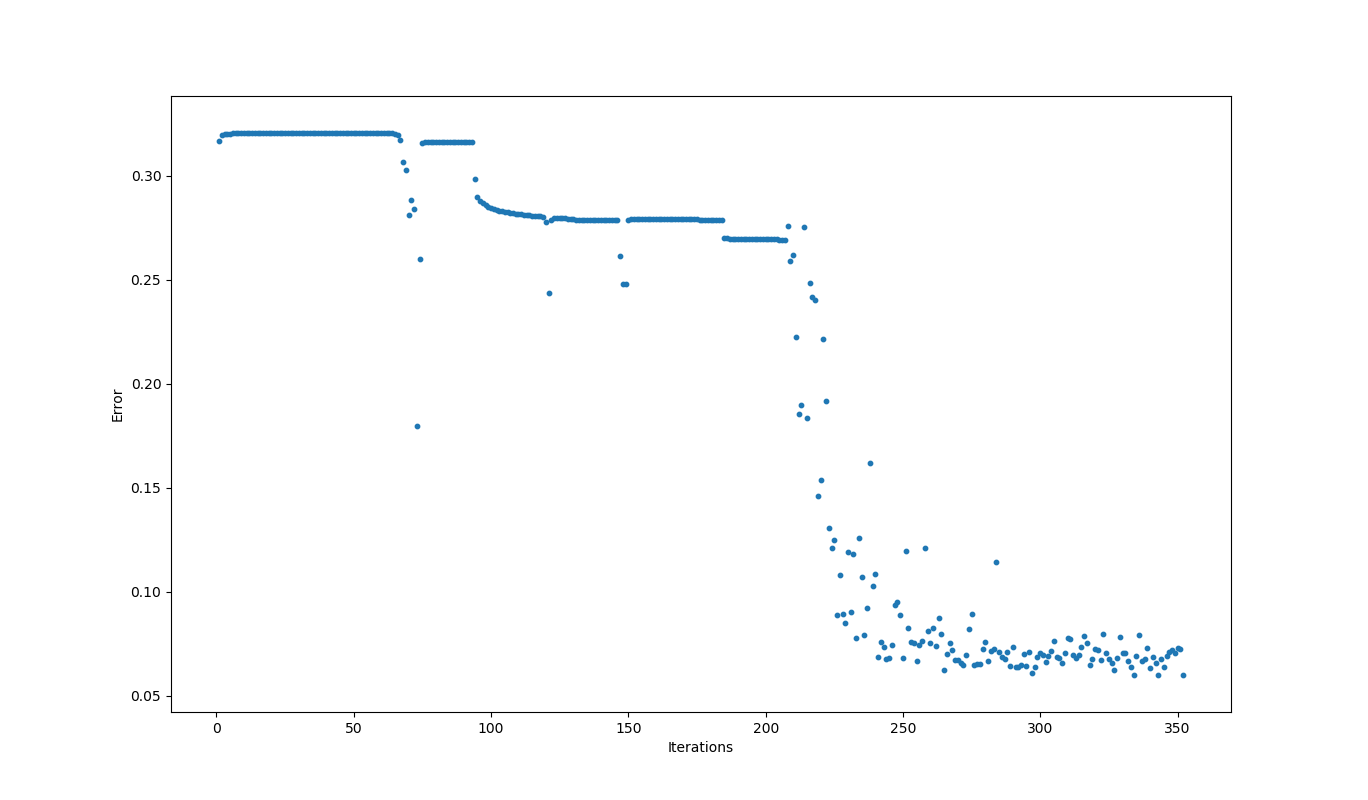
\includegraphics[scale=0.5]{supa_wykres}
\end{document}